\chapter{User documentation}

This chapter provides details on how to install the client application and how to use all of its features. It also explains how to use the server-side API, in case someone would want to build another client application, for example to support the iOS operating system as well.

\section{Client installation}

As we have not yet published the application on the official Play Store, it is necessary to first allow unknown app installation on the used Android device in order to install and use it. This permission needs to be granted to the browser application through which the user wishes to download the app. After this step is performed, the user only needs to visit the application's online repository\footnote{https://github.com/matejsubrt/PragO}, select the desired release of the app and download the \texttt{prago-<version>.apk}\footnote{https://github.com/matejsubrt/PragO/releases/tag/0.1.0} file. After it is downloaded, simply tap the file in the downloads section and follow the installation guide. 

Please note that after first downloading the app, it first needs to download the current data on stops within the network in order to provide stop name suggestions. As this step uses a significant amount of data, it will only be performed when the device is connected to the internet using Wi-Fi. This step may also take a longer time depending on your internet download speed. Thus, we recommend first downloading and launching the app while connected to a Wi-Fi network. Subsequent updates of this data will be performed automatically in the background when connected using Wi-Fi connections and thus do not require any special care.

\section{Client usage}
\label{subsec:usage}

In this section, we will go over the different parts of the application, their user interface and the features they provide.

\subsection{Search screen}

The search screen is the first screen that the user will be presented with after launching the application. It contains the main input fields and most of the toggles and sliders necessary to meet the functional requirements. Only a few settings that are not expected to be changed frequently have been moved to the settings screen.

As you can see in \cref{fig:search_screen}, the search screen contains the inputs for the source and stop names. A click on these leads the user to the stop selection screens, where they can actually select the stop they want. There is also a toggle to flip the direction of the search.

Under the stop name inputs is the row with time settings. First, it contains an icon indicating whether the search is currently set to consider the set time to be the earliest possible departure, or latest possible arrival time. Next to this, the currently set time is displayed. When clicked, this takes the user to the time select screen, where they can select both the time and the departure/arrival setting. Finally, there is a "Now" button at the end that resets the time settings to an earliest departure at the current time.

Under the time row, there is a simple toggle for using shared bikes within the search. 

Finally, there is the section with extended settings. These contain some of the search customization options we decided to provide with our application. The section is minimized by default, but clicking on it reveals its content, as you can see in \cref{fig:extended_settings}. Within this section, the user can set the transfer buffer (corresponds to the \cref{req:transfer_buffer} requirement), the maximum transfer length (\cref{req:max_transfer_distance}) and the balance between shortest time and least transfers (i.e. comfort preference, \cref{req:comfort_balance}). Furthermore, if "Use Shared Bikes" is set to true, this section also contains the slider for setting a bike trip buffer (\cref{req:bike_trip_buffer}) and a toggle to limit the maximum bike trip duration to 15 minutes (\cref{req:bikes_max_15}).

Apart from the source and destination points and the time settings, all other entered values are preserved in between app launches to prevent having to modify them every time the app is being used.

\begin{figure}[h!]
    \centering
    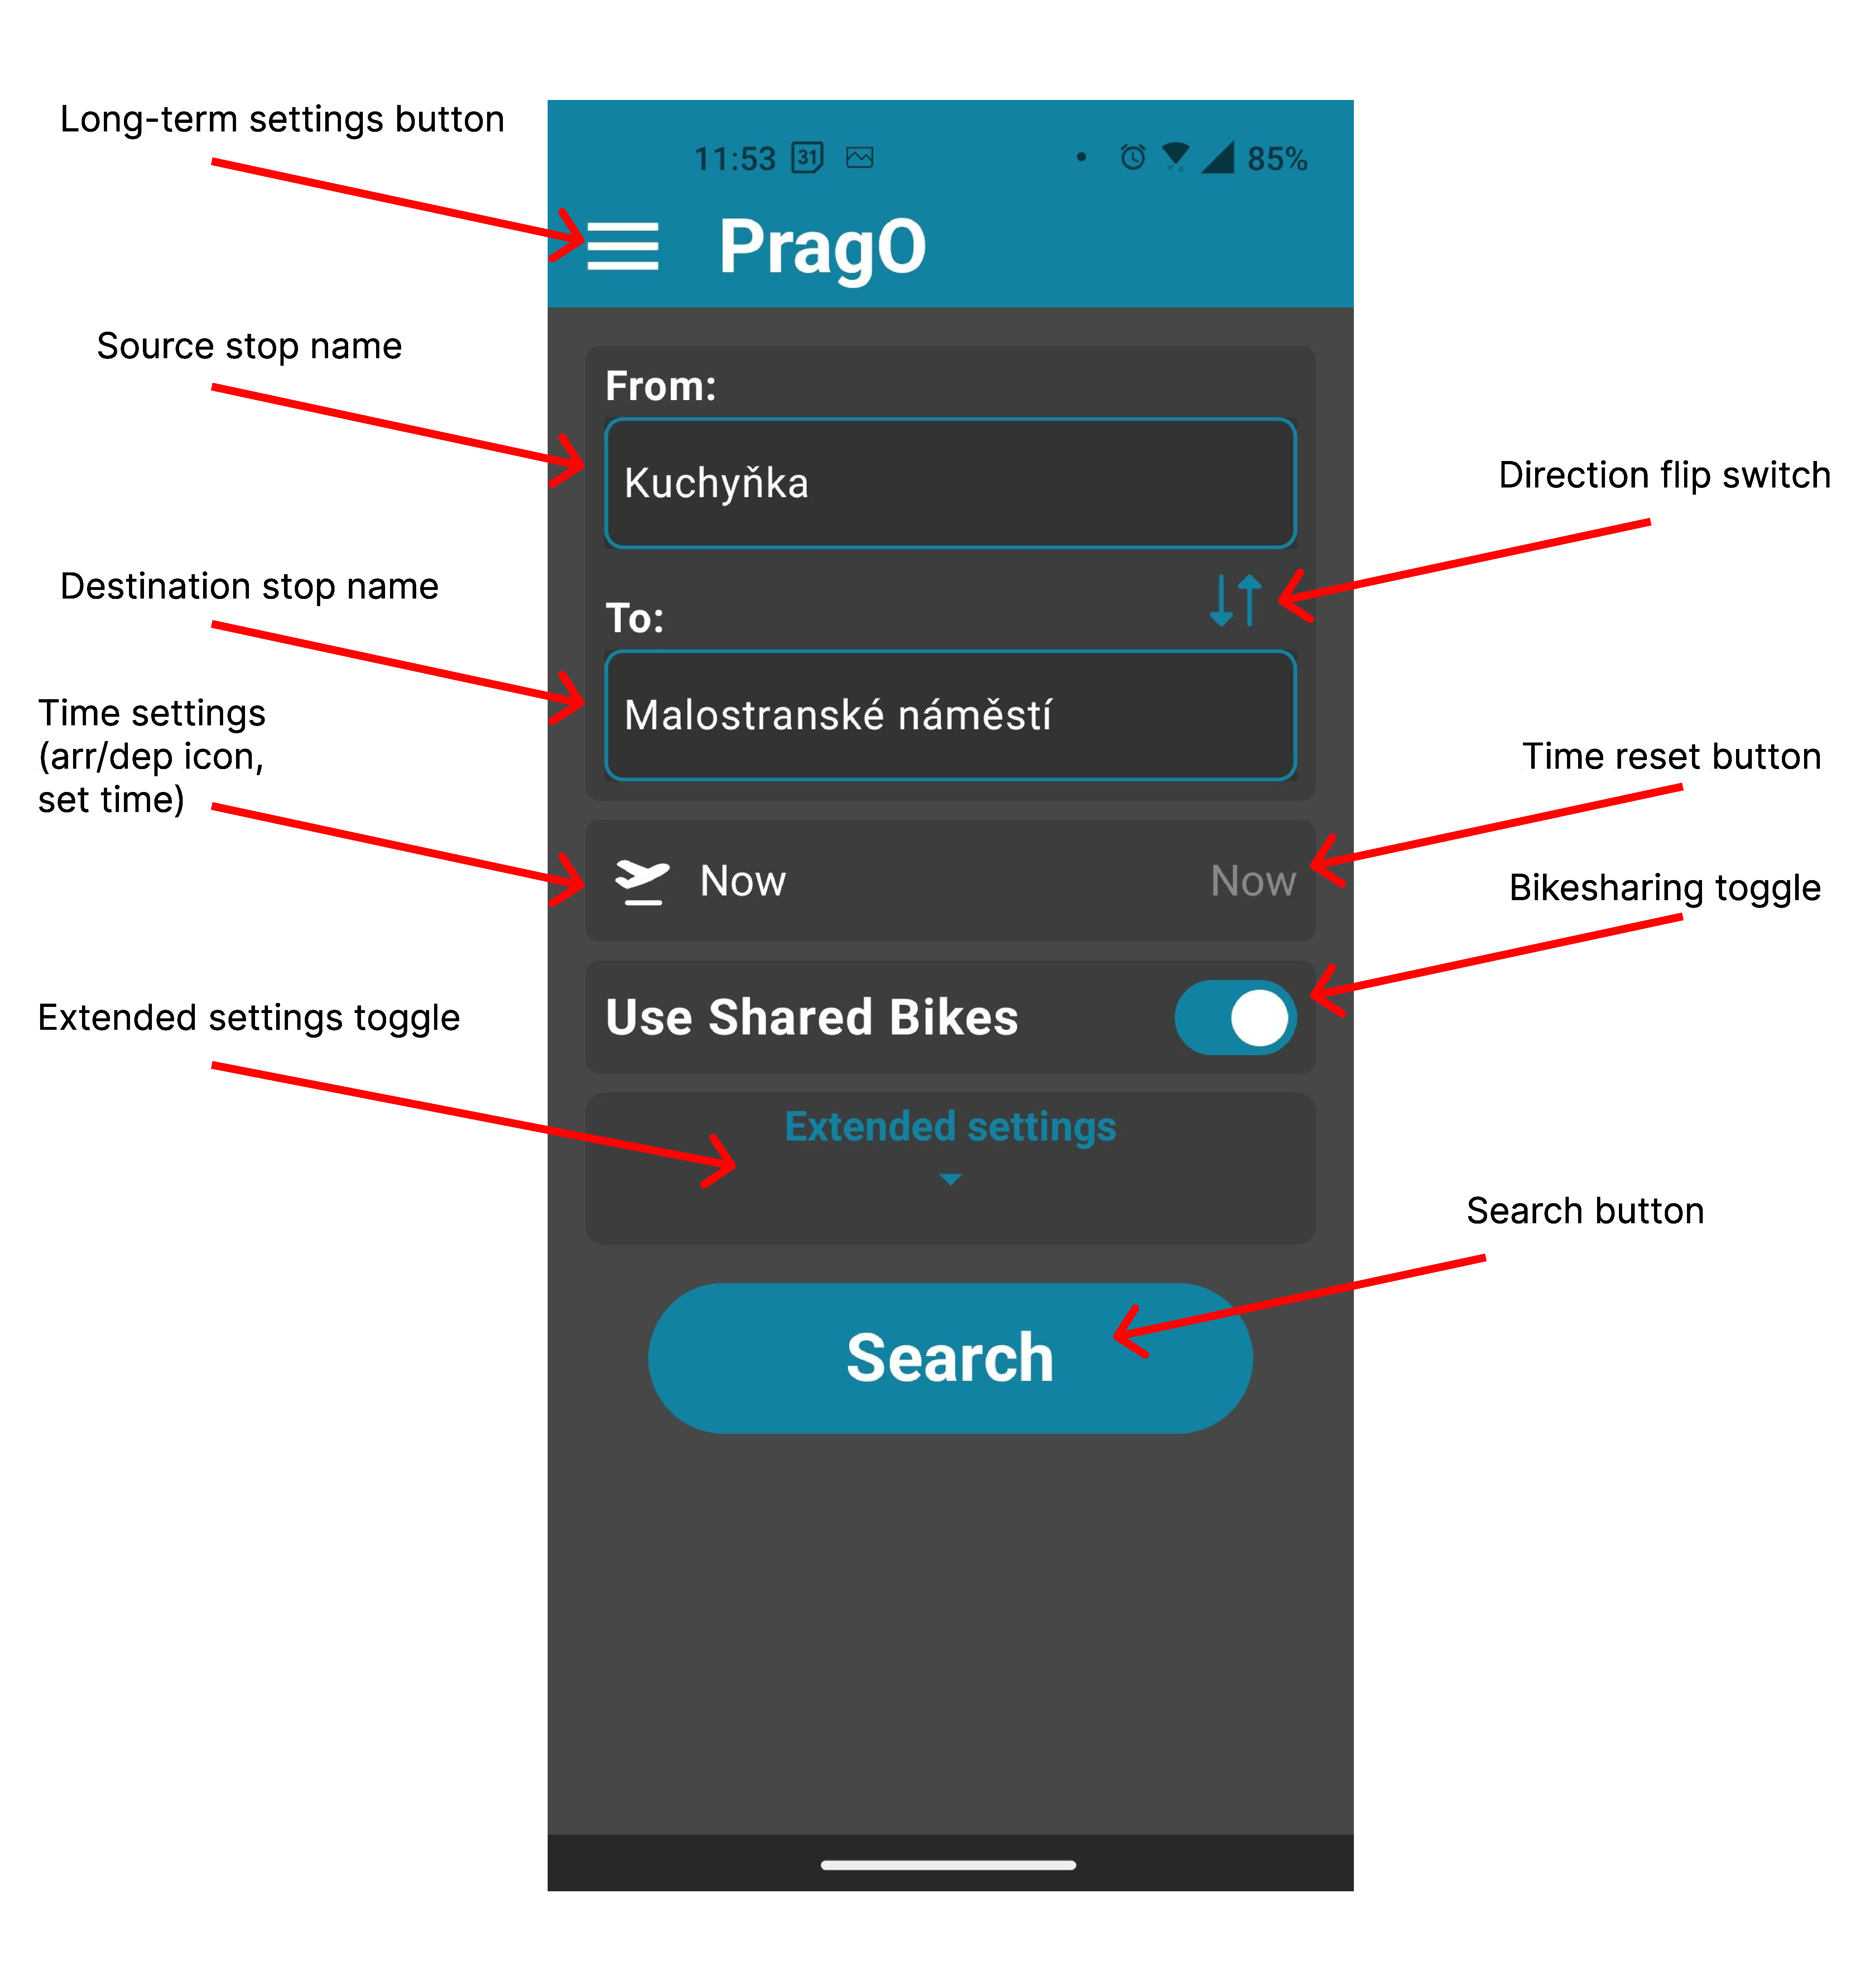
\includegraphics[width=\textwidth]{img/ui_descriptions/search_screen.pdf}
    \caption{Search screen overview}
    \label{fig:search_screen}
\end{figure}

\begin{figure}[h!]
    \centering
    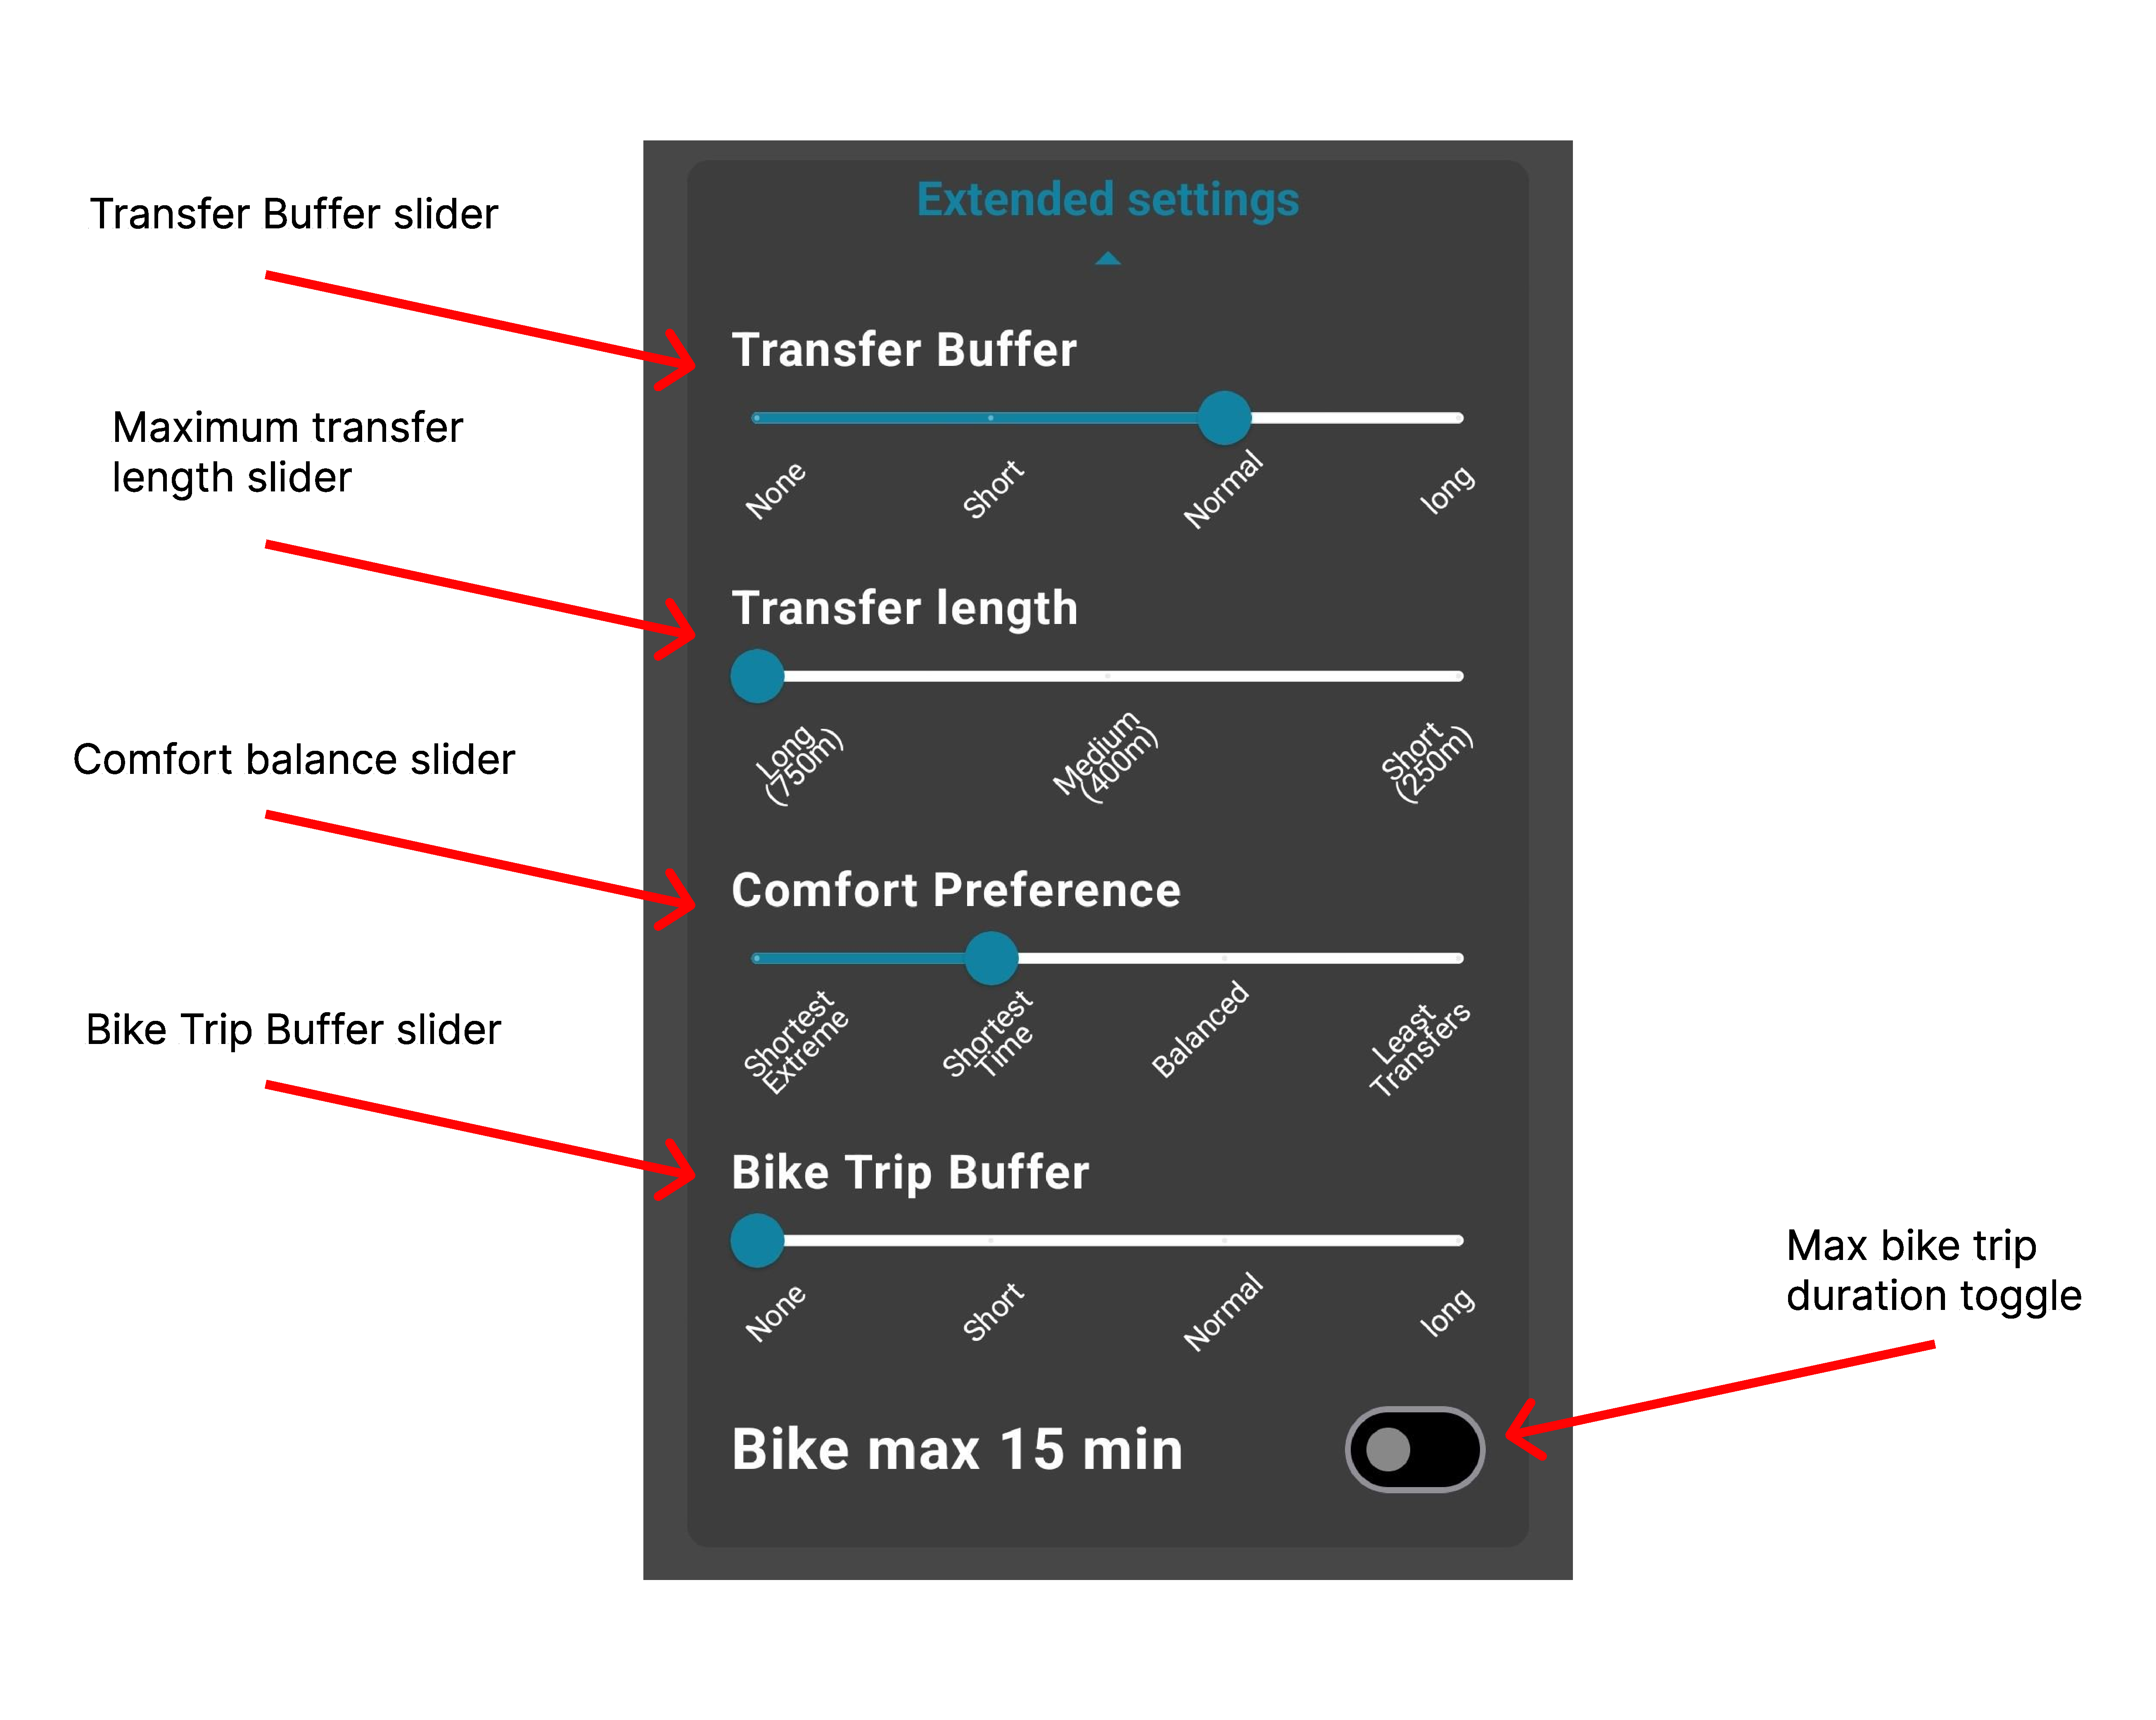
\includegraphics[width=\textwidth]{img/ui_descriptions/extended_settings.pdf}
    \caption{Extended settings section}
    \label{fig:extended_settings}
\end{figure}

\newpage

\subsection{Stop select screen}

This screen (see \cref{fig:stop_select}) will appear when the user clicks on any of the 2 stop selection fields on the search screen. Apart from being able to return back to the search screen via the return button at the top, the user can select the source or destination stops here by typing out their names. The application supports improved searching, which means that for multiple-word stop names, the user can only type the beginnings of each word (i.e. \textit{"mal nam"} for \textit{"Malostranské náměstí"}), and the application will provide the corresponding suggestions (\cref{req:stop_name_suggestions}). Upon clicking on any suggestion, the application saves this preference and returns the user back to the search screen. There is also a delete button that deletes the entered text if the user wants to start from the beginning.

Additionally, when setting the source, the user also has the opportunity to select the "My location" suggestion, which will start the search using the user's current coordinate location instead of using a stop name (\cref{req:src_by_coords}). Note that for this to work, the user must allow the application to use their location in the popup that will appear.

\begin{figure}[h!]
    \centering
    \includegraphics[width=\textwidth]{img/ui_descriptions/stop_search_screen.pdf}
    \caption{Stop select screen}
    \label{fig:stop_select}
\end{figure}

\newpage


\subsection{Time select screen}

On this screen (see \cref{fig:time_select}), the user can adjust all the time settings. They can change the date via the date setting wheel, the time via the time setting wheel and the meaning of the selected time, i.e. whether it sets the earliest departure or latest arrival boundary (\cref{req:arr_dep_time}). Upon clicking the "Done" button, the user is taken back to the search screen.

\begin{figure}[h!]
    \centering
    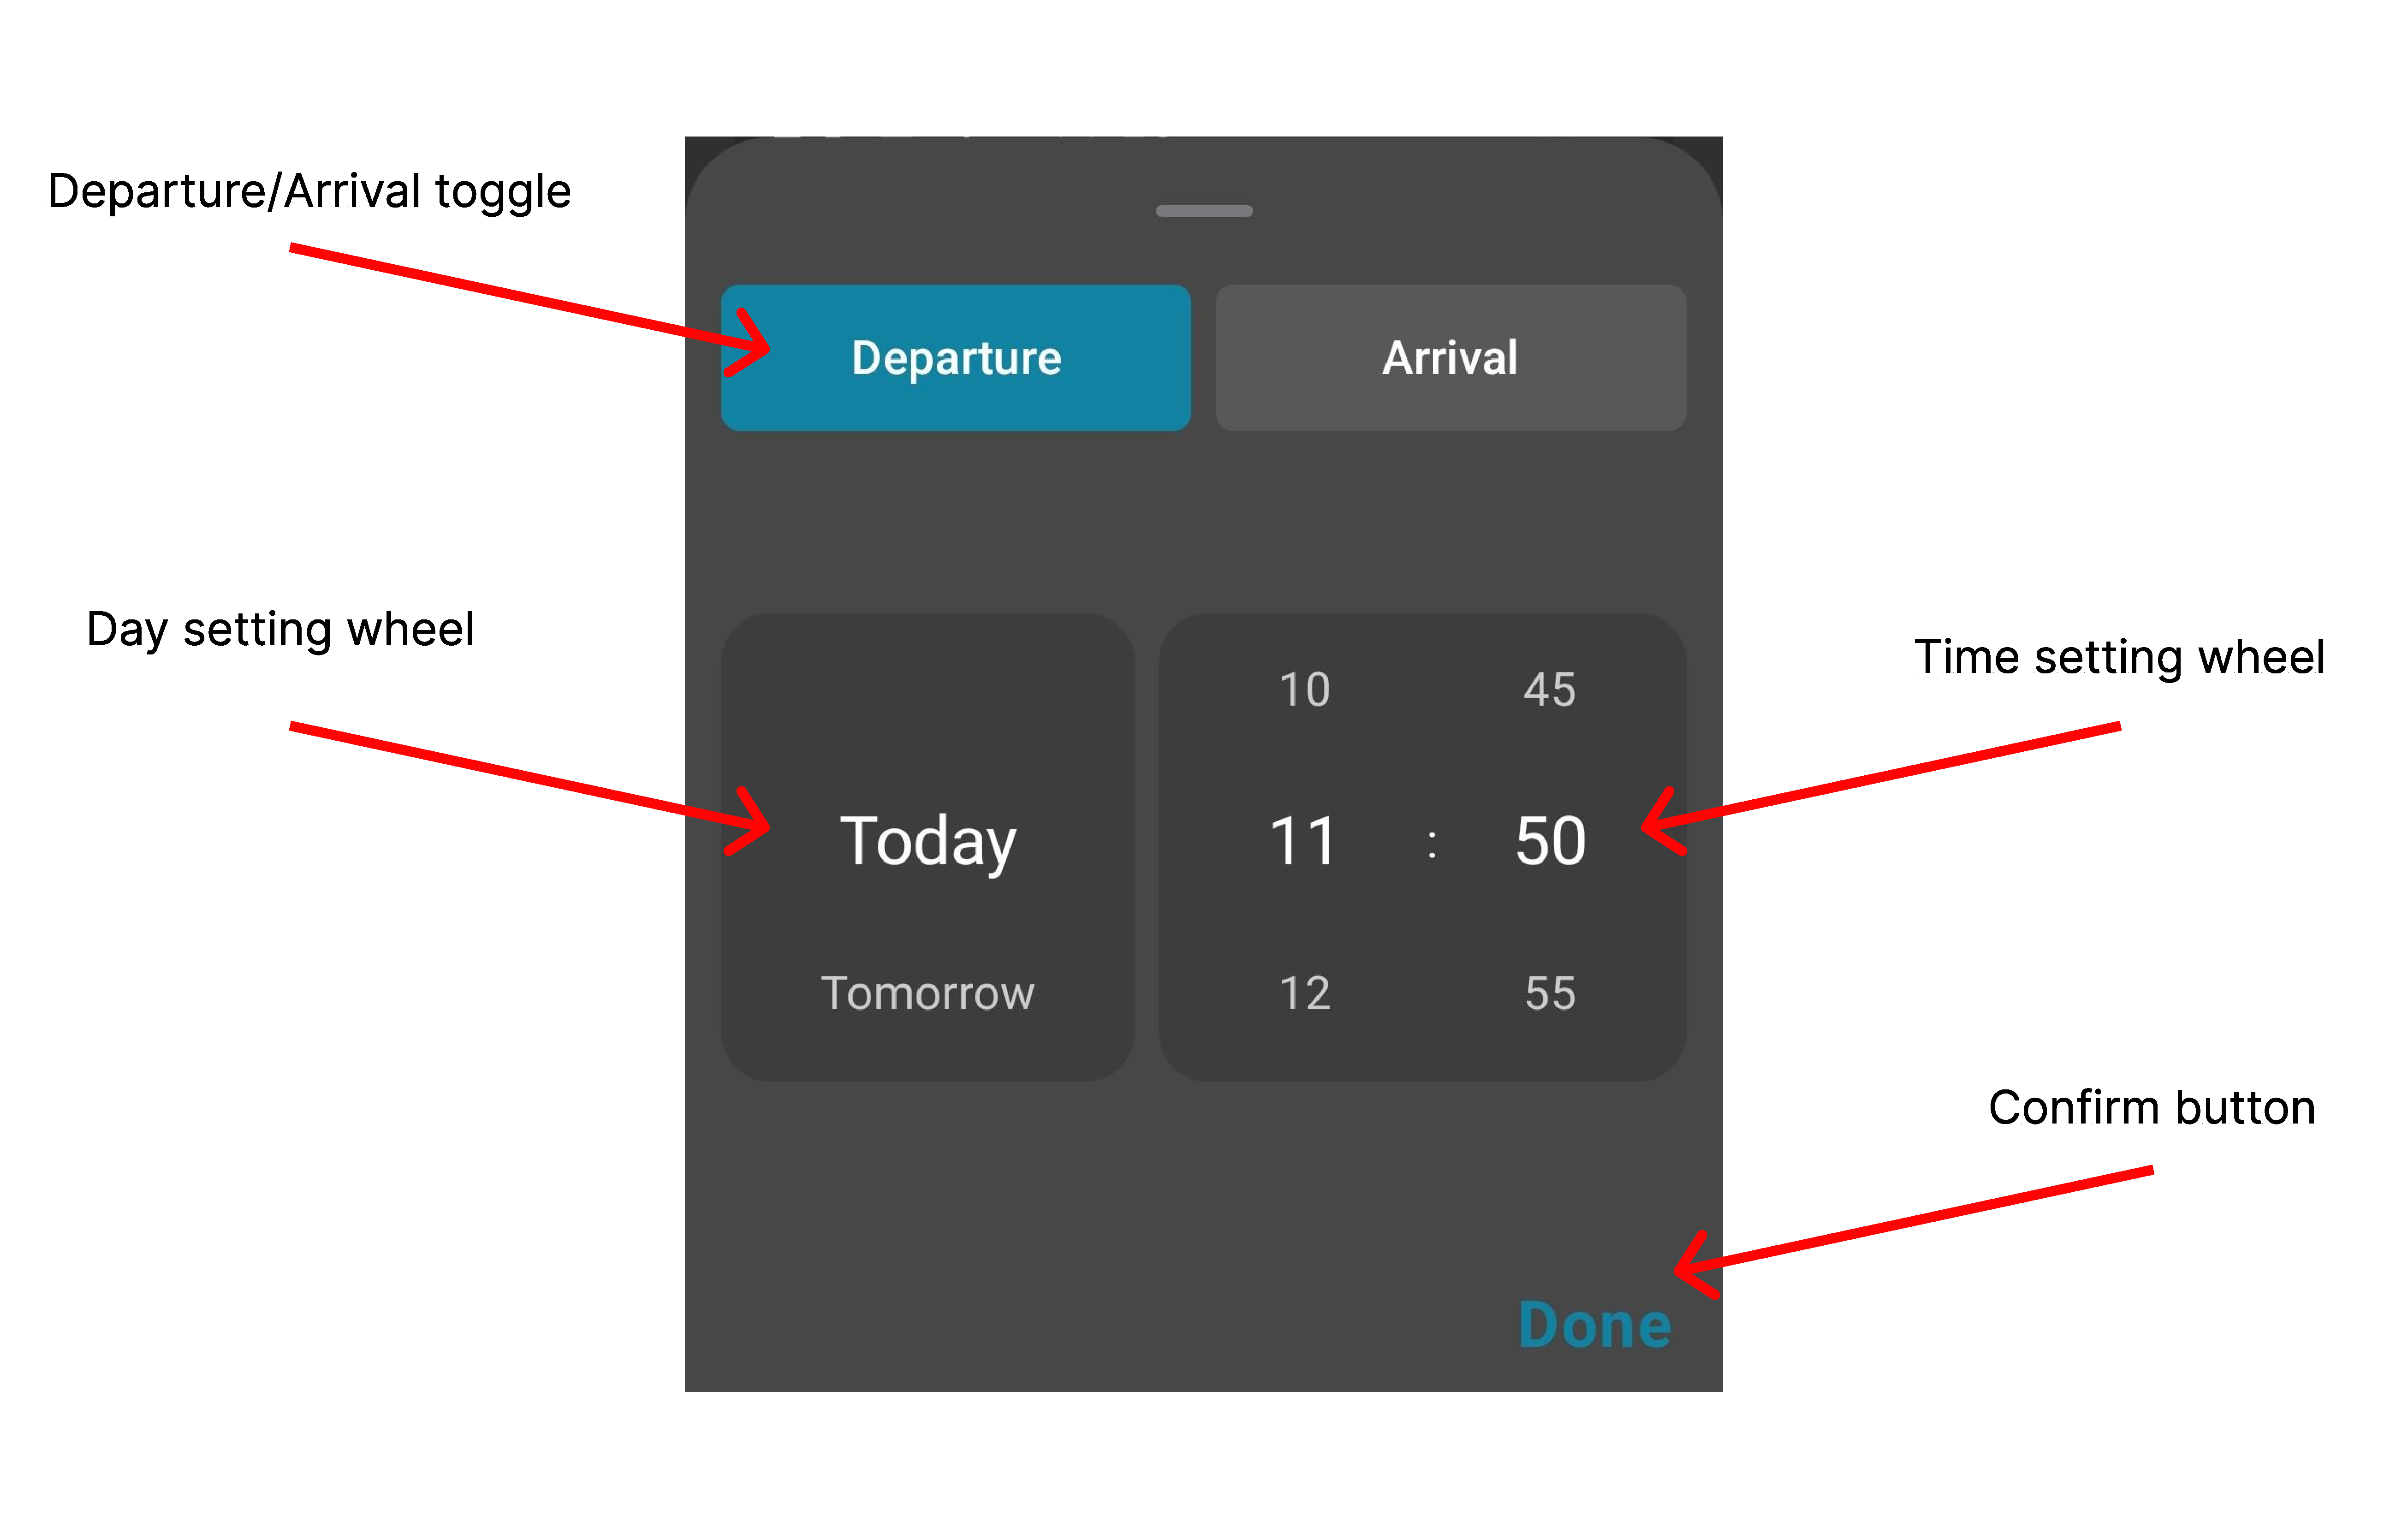
\includegraphics[width=\textwidth]{img/ui_descriptions/time_settings.pdf}
    \caption{Time select screen}
    \label{fig:time_select}
\end{figure}

\newpage

\subsection{Settings screen}

This screen provides access to all the settings that typically do not change very often and thus do not need to be included on the main search screen. As you can see in \cref{fig:settings_screen}, these include setting the walking pace (\cref{req:walking_pace}), cycling pace (\cref{req:cycling_pace}) and the shared bike lock and unlock times (\cref{req:lock_unlock_time}). By clicking the "Save and return" button, the user saves the values and returns to the search page.


\begin{figure}[h!]
    \centering
    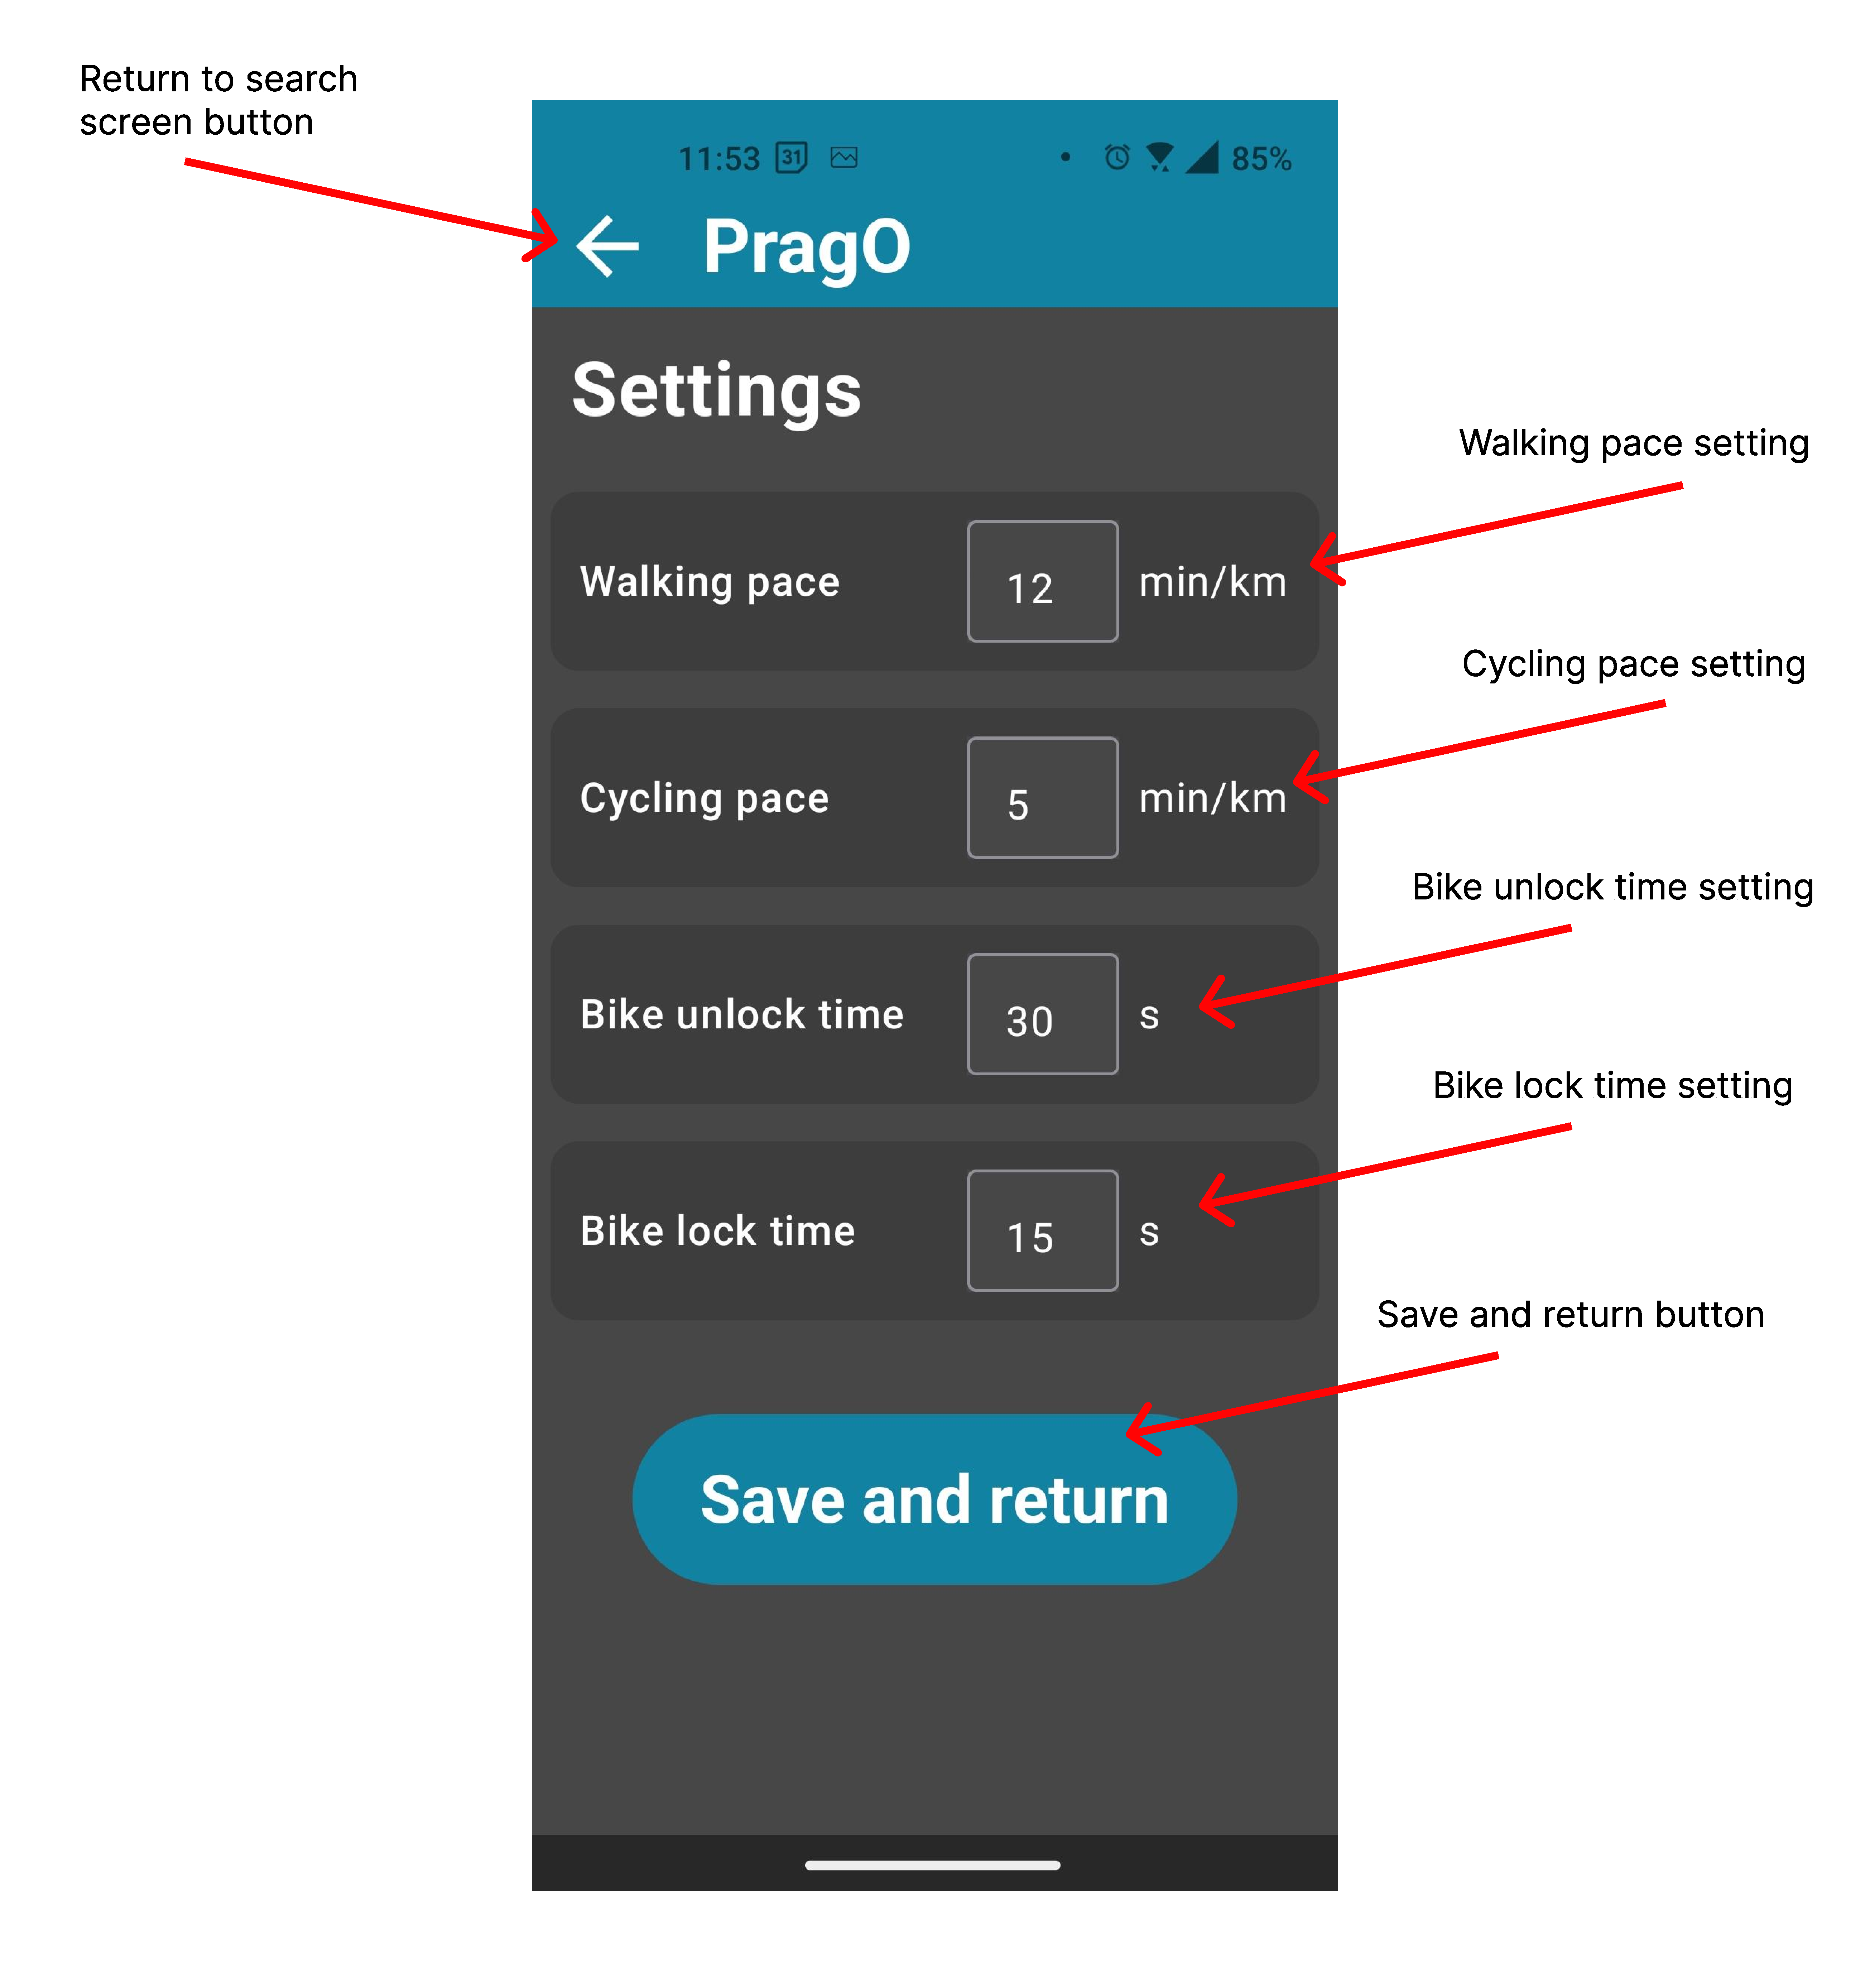
\includegraphics[width=\textwidth]{img/ui_descriptions/settings_screen.pdf}
    \caption{Settings screen}
    \label{fig:settings_screen}
\end{figure}

\newpage


\subsection{Results screen}

This is where the results of the search get displayed. According to requirement \cref{req:multiple_results}, our app does not just search for a single connection, but rather searches for multiple best connections across a time range. In particular, the app first searches for the best connection according to the given parameters. Then, if the user scrolls further down the page, it loads further later connections. If the user wants to view earlier connections, they can pull down while on top of the page, which will expand the results into the past.

Every individual result is displayed in the form of a single connection card. As you can see in \cref{fig:results_screen}, this card contains all the necessary information about all the segments of the connection. At the top, there is a countdown until the connection leaves and the total duration of the connection (\cref{req:countdown}). Furthermore, the countdown has 3 variations - in cases, where the connection immediately begins by boarding a trip at the source stop, only a countdown until boarding the trip is displayed (see "Time until first departure" in \cref{fig:results_screen}. In cases where the connection only consists of transfers and bike trips, there is no time limitation as to when the connection may be performed. Thus, such connection are marked as "Anytime" (see "Departure possible anytime" in \cref{fig:bike_results}). Finally, in cases where the connection begins with a transfer and later down the line continues with a trip, two countdowns are displayed - one showing the time left until the first trip leaves and a second one showing the time left until the user should start the initial transfer (see "Time until initial transfer start" in \cref{fig:results_screen}). If the first trip has not yet departed, but the time at which the user was supposed to start walking to make the connection has already elapsed, the first trip countdown is highlighted to remind the user of this situation (see "Time left until first trip departure" in \cref{fig:bike_results}).

Every segment within the connection then has a separate section within the result card. For a trip, the line name, together with the boarding and disembarking stops and exact times (\cref{req:exact_times}) and the current delay (\cref{req:delays}) of the trip are displayed. For a transfer, the distance and expected duration are shown. Finally, for a bike trip, the application displays its source and destination bike stations' names, the distance and expected duration of the trip, and the current number of free bikes available at the source station (\cref{req:bike_count}) (see \cref{fig:bike_results}).

The user can also swipe left or right on any of the displayed public transit trips to reveal its earlier/later alternatives (\cref{req:trip_alternatives}). It is also possible to click on any of the displayed bike trips, which (when connected to the internet) will take the user to the Mapy.cz application and display the route they are supposed to take. Note that the length of this displayed route might vary slightly from the distance specified in our app, as we use a different routing engine and map data for our searches.

\begin{figure}[h!]
    \centering
    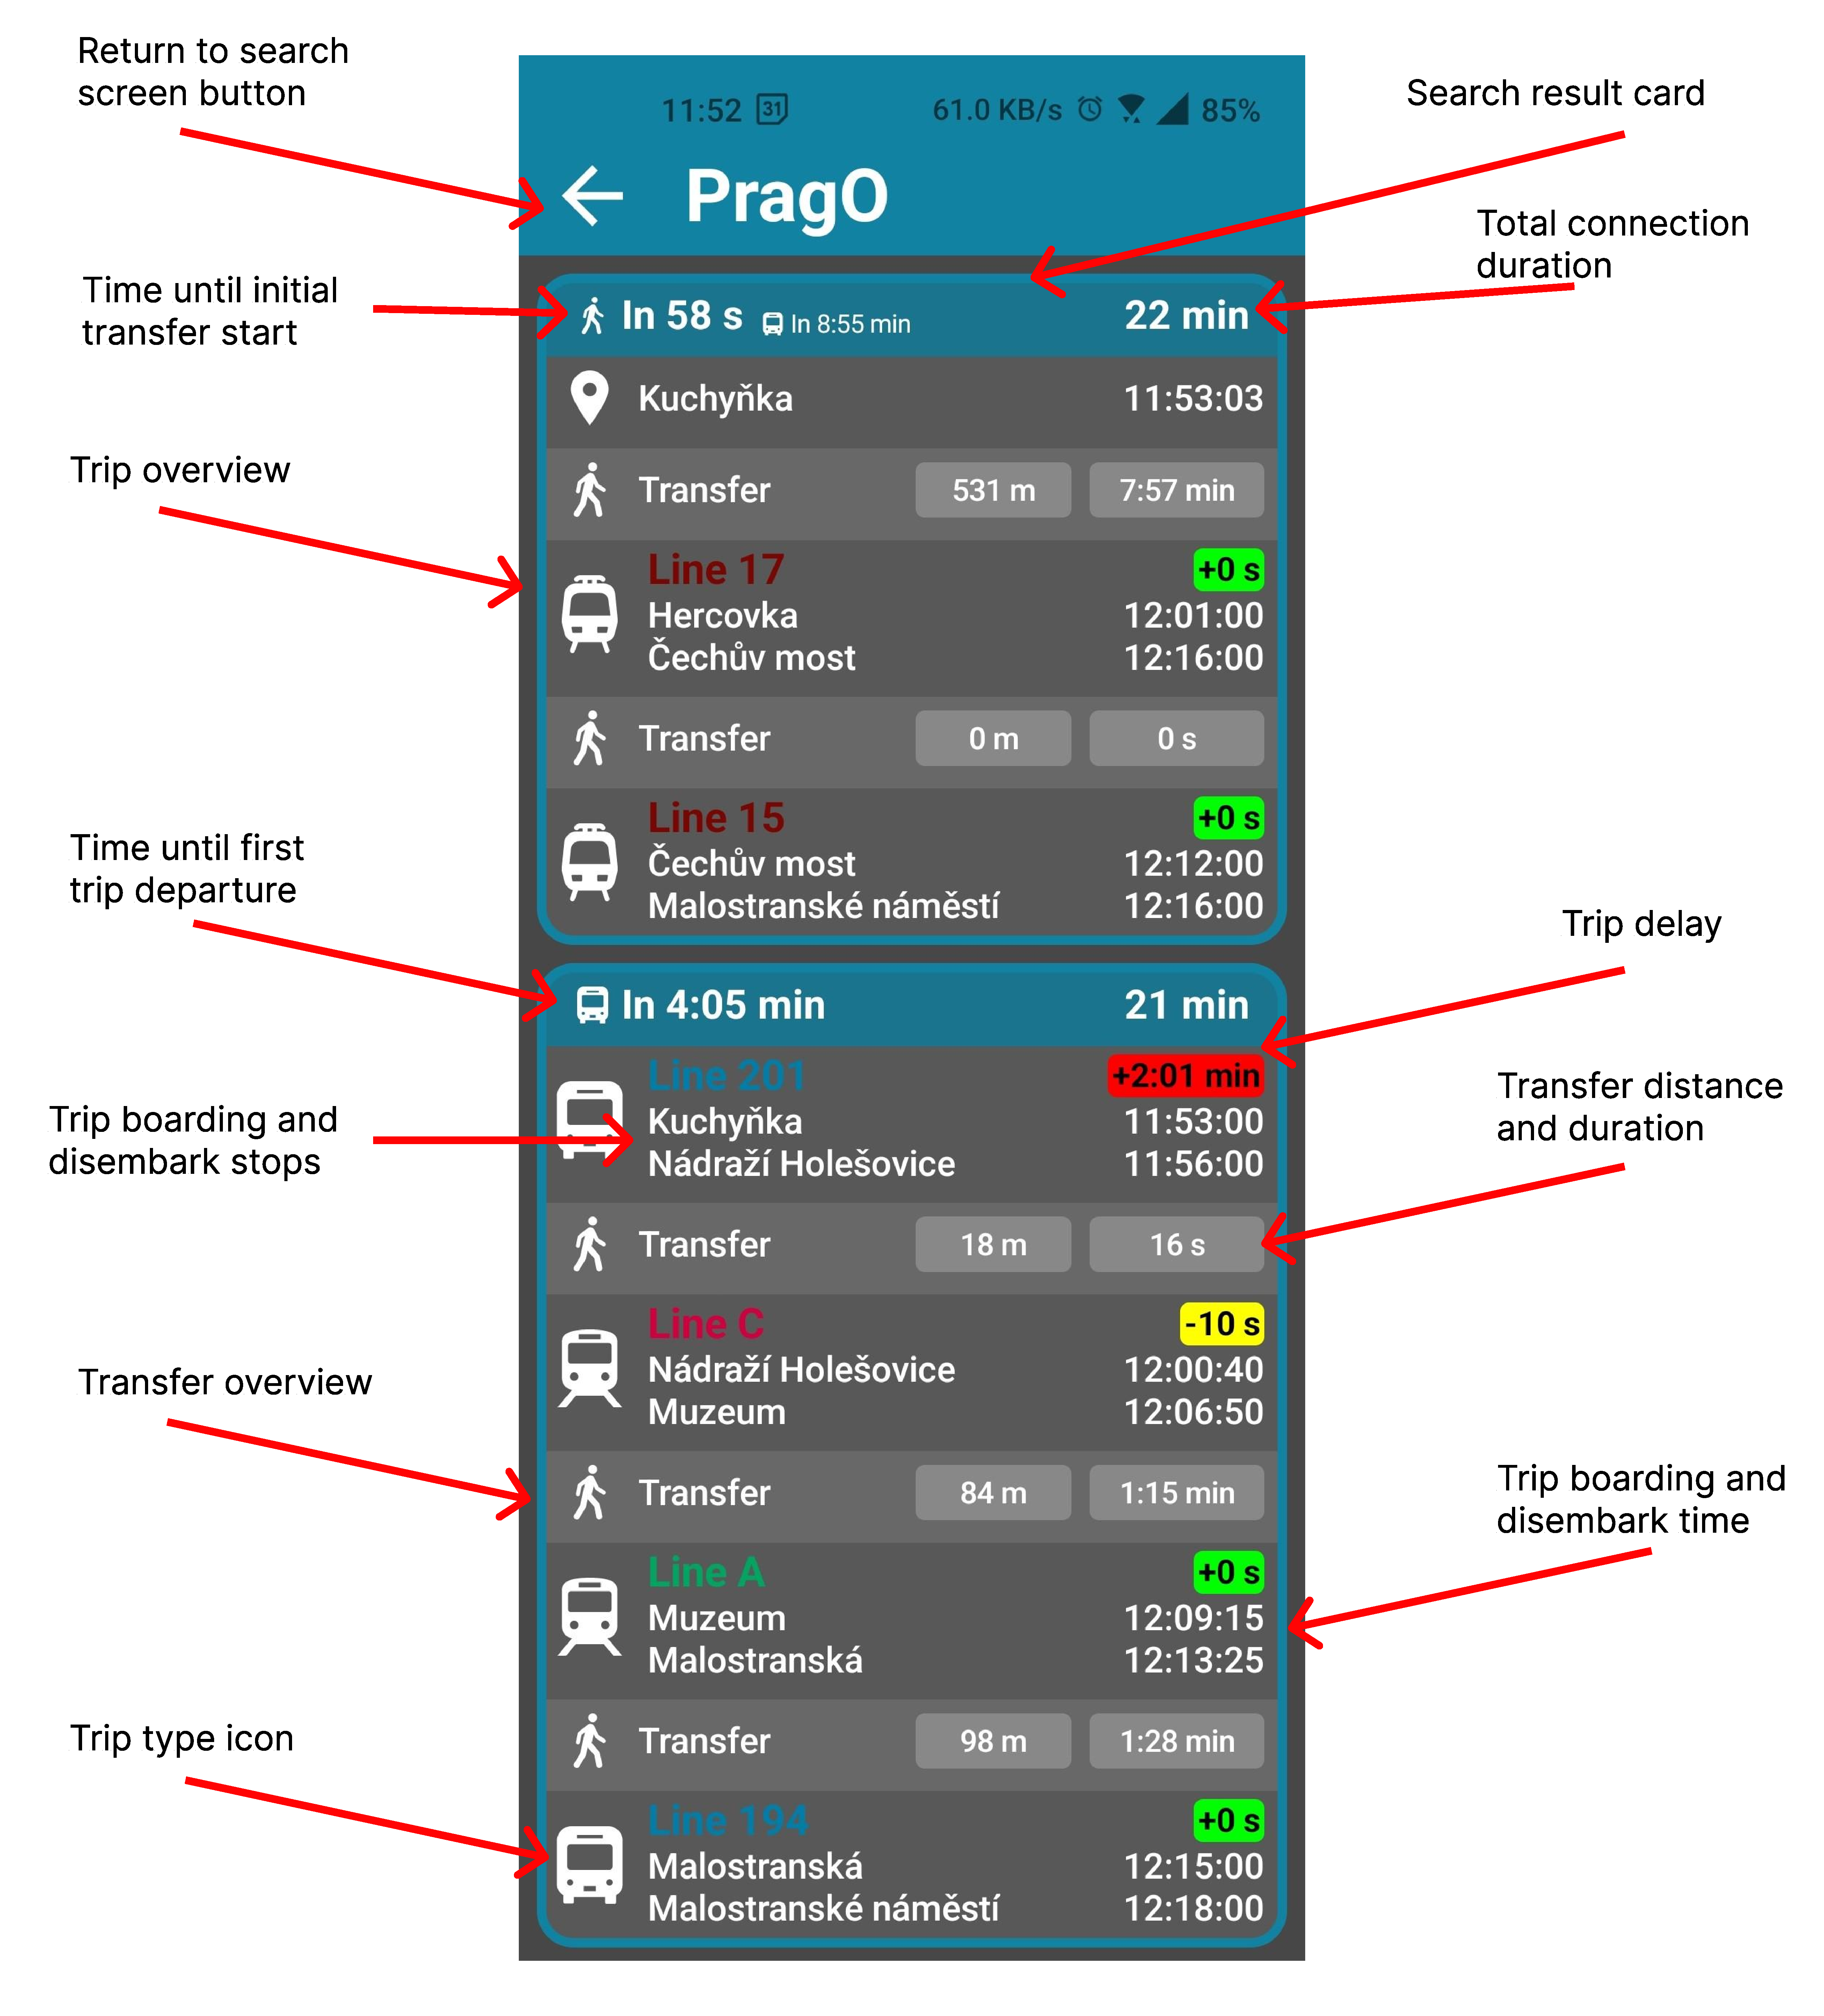
\includegraphics[width=\textwidth]{img/ui_descriptions/result_screen.pdf}
    \caption{Results screen}
    \label{fig:results_screen}
\end{figure}

\begin{figure}[h!]
    \centering
    \includegraphics[width=\textwidth]{img/ui_descriptions/bike_results.pdf}
    \caption{Bike result cards}
    \label{fig:bike_results}
\end{figure}


\section{API usage}

Apart from using the provided client application, it is also possible to use the back-end API directly. There are 3 distinct POST endpoints - a connection search endpoint, a trip alternatives endpoint and a delay updating endpoint. Let's go over them and explain their purpose. Note that when running the server-side application in the WebAPI (and not WebAPI-light) configuration, the exact schemas of the requests and responses, as well as other information about the API, can be found on the address \texttt{<BASE-URL>/swagger/index.html}, so we will not be showing them here.

\subsubsection{Connection search endpoint}
\label{subsec:connection_endpoint}

The connection search endpoint at the address \texttt{<BASE-URL>/connection} is the main endpoint for connection searching. It takes a connection request object containing all the search parameters including the source and target locations, the specified time and the settings for the search. It returns a list of the first relevant connections for the search parameters. This endpoint is also used for search expanding - in case the client already has some results and wants to request later ones, it can send the same request with the time set to the departure of the last existing result and the \texttt{byEarliestDeparture} parameter set to \texttt{true}. Analogically, when expanding to the past, time is set to the arrival time of the earliest existing connection and \texttt{byEarliestDeparture} to \texttt{false}.

This endpoint may respond with the codes \texttt{200: OK} if the connection was successfully performed, \texttt{404: Not Found} in case no connection was found for the parameters and \texttt{400: Bad Request} in case any of the provided parameters or setting values were invalid. In that case, the response will contain a message with the reason for the failure.

\subsubsection{Trip alternatives endpoint}

This endpoint exists at the address \texttt{<BASE-URL>/alternative-trips} and serves the purpose of finding alternative direct trips. The client needs to provide the ids of 2 stops between which direct trips run and the id of the trip for which it wants to find the alternatives, a time and a parameter specifying whether to find earlier or later alternatives. The API will then respond with a list of alternative direct trips. Once again, the possible response codes are \texttt{200: OK} if found correctly, \texttt{400: Bad Request} when some of the parameters were invalid or \texttt{404: Not Found} when the alternative trips could not be found.

\subsubsection{Delay updating endpoint}

\xxx{Hasnt this changed???}

This endpoint at the address \texttt{<BASE-URL>/update-delays} has the same input and output parameter. It takes a list of existing results, goes through all trip alternatives of all trip segments of all the results and updates all their delay data. Then it returns these newly updates results. This endpoint only returns the code \texttt{200: OK}, as it discards results which it cannot process.